\section{\Thehostabi{} efficiency}


%The efficiency of \hostapis{} directly impacts the performance of \graphene{} on each host.
%A large portion of \linuxapis{} inside \thelibos{} require resources or abstractions from the host OS.
%Since \thehostabi{} is the only interface for requesting host OS features,
%the definition of \thehostabi{}
%restricts the options for a \picoproc{} to optimize its own performance, according to the application's performance patterns.
%Although each PAL may optimize individual \hostapi{} for general circumstances,
%all applications must share the same PAL ABI and thus tolerate the same overheads of exporting these \hostapis{} on each host.



The section evaluates the efficiency of \thehostabi{} in comparison with
the underlying host system interfaces.
The implementation of \thehostabi{} is independent
for each host where \graphene{} is ported,
and therefore shows different
performance patterns on each PAL.
Upon a certain host, the base latency of a \hostapi{} is mostly determined by the host \linuxapis{} or abstractions
chosen to implement such \hostapi{}.
%Three primary factors determine the efficiency of \hostapis{}.
%First, especially on Linux or other monolithic OS,
%most of \thehostabi{} are directly translated to similar \linuxapis{}.
%The efficiency of these \hostapis{}
%are dominated by the basic cost of the host system interface,
%and the performance of corresponding \linuxapis{}.
For instance, on a Linux host, the latency of \palcall{StreamRead} is comparable to the latency of \syscall{read},
since the former is essentially
a wrapper of the latter.
If a \picoproc{} runs inside an SGX enclave,
the latency of \palcall{StreamRead} is approximately the same as the turnaround time of exiting the enclave,
invoking a \syscall{read} \linuxapi{}, and returning the contents back to the enclave.
The latency on the SGX PAL is then mostly dominated by the overheads
of switching the context between the enclave
and the untrusted, external PAL using SGX instructions,
and bringing memory into the EPC (enclave page cache).
% or decrypting memory on a last-level cache miss.


In theory, the design of \thehostabi{}
is meant to minimizing the overheads of translation to most host system interfaces.
Since most \hostapis{} are just wrappers
of the underlying \linuxapis{},
the translation cost is mostly reduced to simply replacing the generic identifiers and control flags
to the semantics that are recognized by the host OS.
A common operation
for the translation is to scan a URI (unified resource identifier), such as file or network URI,
and compose a equivalent file system path or network address
for the host OS.
%The second factor is the translation cost
%of the \hostapis{}.
%For portability, \thehostabi{} is defined with generic semantics, without host-specific notions
%such as process identifiers, file descriptors,
%file system paths,
%and \linuxapi{} flags.
%The PAL must translate the arguments of \hostapis{}, including PAL handles, URIs (Uniform Resource Identifiers), and generic flags,
%to the arguments interpretable by the host kernel.
These translation costs
are relatively marginal and deterministic, compared to the overall latency of a \hostapi{},
because the translation is mostly straightforward,
and only requires simply logics
and little memory copy.
Without extra security checks,
a \hostapi{} is more likely to suffer high overheads if the implementation
requires additional \linuxapis{} for complementary operations
to the base abstraction,
or constantly retrying a \linuxapis{} at failures.



More significant overheads
on a number of \hostapis{} contribute to security checks or enforcements,
for ensuring the safety of running an application
within the threat model
of a host.
%Finally, the third factor that impacts the PAL call efficiency
%is the cost of security checks,
%either inside the host kernel or the guest.
%The cost of security checks varies between hosts, and is correlated with the presumed security models.
On a Linux host, the security model
focuses on isolating mutually-untrusting applications,
therefore requires checking
the \hostapis{} in the Linux kernel,
to restrict the sharing of host resources and unpermitted system interfaces,
using both the reference monitor and \seccomp{} filter.
Inside an SGX enclave, the security checks
for the \hostapis{}
protects the application and \libos{} from an untrusted OS,
and thus focus on validating the results of \linuxapis{},
using either cryptographic techniques or semantic checks.
Cryptographic techniques are used to: (1) validate the file against the secure hash, at \palcall{StreamOpen}, (2) check the file chunks against a Merkle tree of hash values, at \palcall{StreamRead}, and (3) establish a TLS connection over inter-enclave RPC, at \palcall{ProcessCreate}.
For the SGX PAL,
the latency of a \hostapi{} can be dominated
by the cost of cryptographic operations,
on large chunks of data exported to the untrusted OS.


The evaluation in this section is based on micro-benchmark programs similar to \lmbench{} 2.5~\cite{McVoy:lmbench}.
For each \hostapis{}, the evaluation also shows the breakdowns
of its latency or throughput,
by benchmarking the PALs both with and without the security mechanisms, such as the \seccomp{} filter and reference monitor on the Linux PAL,
as well as testing under different
implementation strategies.
The evaluation focuses on \hostapis{} that are especially sensitive for the performance of the \graphene{} \libos{}.


% the efficiency of \hostapis{} on both Linux and SGX hosts, and shows the impact of each performance factor.
%The evaluation is based on micro-benchmark programs similar to \lmbench{} 2.5~\cite{McVoy:lmbench},
%and is compared against
%similar \linuxapis{} on Linux.



\subsection{Stream I/O}

This section separate the evaluation of stream I/O in \thehostabi{} into 
%The \hostapis{} for stream I/O can be separated into 
two categories:
(1) file system operations and (2) I/O operations on a network socket or a RPC stream.
The evaluation for file system operations
primarily measures
the latency of retrieving file metadata from the storage or a host kernel file system directory cache,
as well as the latency of sequential reads or writes
inside a regular file.
%access a UNIX-style, hierarchical, host file system,
%with either random access to file contents,
%or access to file attributes (metadata).
The evaluation for other I/O streams, such as a network socket or a RPC stream,
then focuses on measuring the latency or bandwidth
of sending and receiving messages 
across \picoprocs{} or applications.

%over a network address or a local, in-kernel queue.
%Due to the difference in the nature of these operations,
%the evaluation separates
%file access from network or RPC workloads.






\paragraph{Opening a file.}
The evaluation shows the latency of identifying a file inside the host storage and attaching the file resources to the running application. 
Figure~\ref{fig:eval:pal:open-latency} (a) and (b) shows the latency of \palcall{StreamOpen} on the Linux and SGX PALs,
in comparison with \syscall{open} in a native Linux process.
Because the micro-benchmark
(based on \lmbench{})
primarily measures the latency of repeatedly opening the same file, the results are subject to the cost of
the file system directory cache inside the host kernel,
without almost no cache misses.
\citeauthor{tsai15dcache}~\cite{tsai15dcache}
shows that, with a warm cache,
the latency of a file-searching \linuxapi{} on Linux,
such \syscall{open} or \syscall{stat}, 
is strictly correlated with
lengths and depths of the requested paths,
because the lookup functions of the current file system directory cache design
are based on searching each path components
(i.e., directory names separated by the common slash character)
inside a hash table.

\begin{figure*}[t!]
\centering
\footnotesize
\resizebox{\textwidth}{!}{%
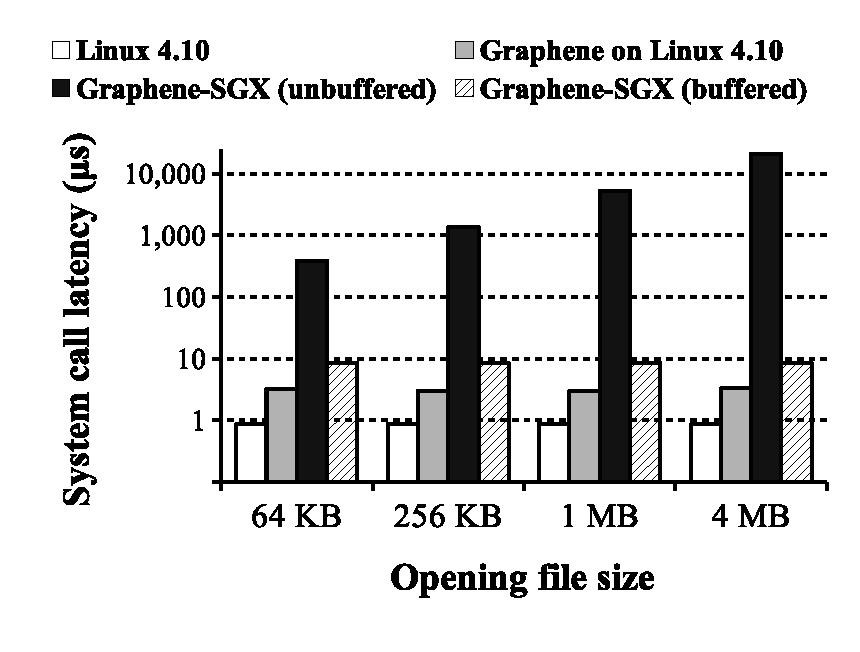
\includegraphics[height=10em]{pal/open-latency}
\quad
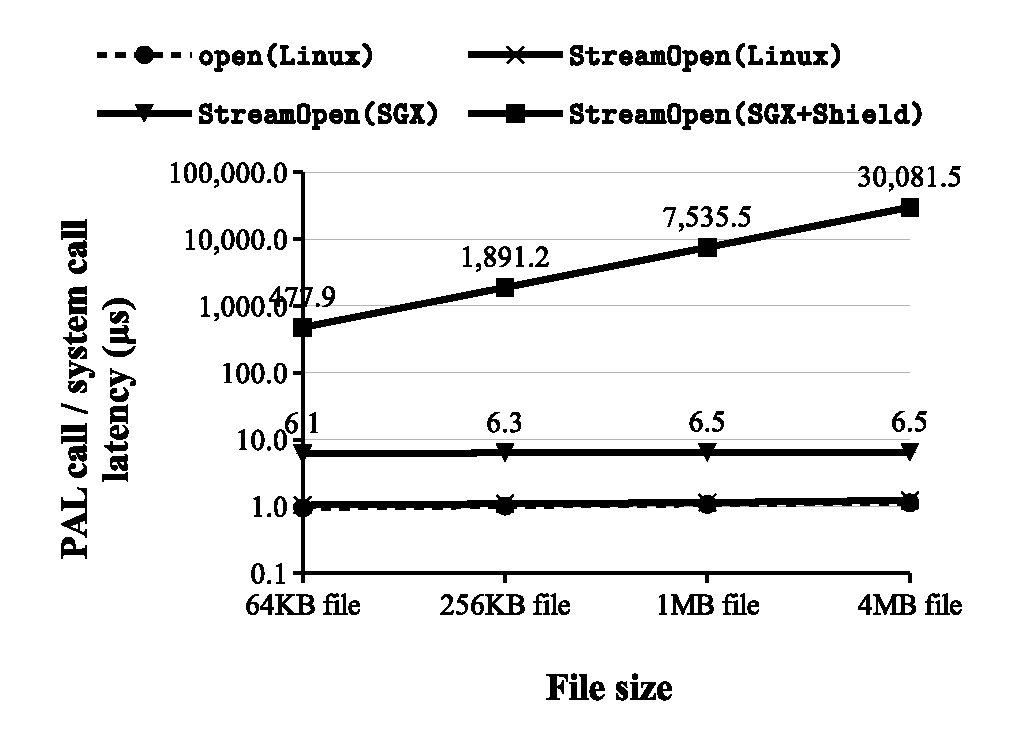
\includegraphics[height=10em]{pal/sgx-open-latency}
}
\parbox{0.49\textwidth}{\centering\bf (a) Linux vs. Linux PAL}
\parbox{0.49\textwidth}{\centering\bf (b) Linux vs. Linux PAL vs. SGX PAL}
\caption{Latency of \palcall{StreamOpen} on the Linux PAL  and SGX PAL, versus \syscall{open} on Linux.
Lower is better.
Figure (a) compares \palcall{StreamOpen} on the Linux PAL,
with and without a \seccomp{} filter ({\bf +SC})
and reference monitor ({\bf +RM}), against \syscall{open} on Linux. Figure (b) compares \palcall{StreamOpen} on a SGX PAL,
with and without integrity checks ({\bf +CHK}),
against the Linux PAL and \syscall{open} on Linux.}
\label{fig:eval:pal:open-latency}
\end{figure*}

Figure~\ref{fig:eval:pal:open-latency} (a)
shows a similar pattern for \palcall{StreamOpen}
on the Linux PAL,
because \syscall{open} is used as the underlying host \linuxapi{}. %of \palcall{StreamOpen}.
The translation cost between \palcall{StreamOpen} and \syscall{open} is merely 6--10\%,
primary caused by scanning the file URIs and translating
the control flags of \palcall{StreamOpen}
to Linux \linuxapi{} flags.
The \seccomp{} filter adds 7-10\% overheads, or \roughly{}0.9 \usec{}, to the latency of \palcall{StreamOpen}, with JIT (Just-in-time) optimization. Finally, if the reference monitor is enabled, the reference monitor adds an extra 14-21\% overheads, and the overheads are roughly correlated with the length of requested paths.
The overhead of the reference monitor
is caused by redirecting \syscall{open} \linuxapis{} through \syscall{ioctl}, and checking the paths against the file access rules written inside the manifest of the running application.  












Figure~\ref{fig:eval:pal:open-latency} (b) shows the latency of \palcall{StreamOpen} inside of an SGX enclave, versus the latency on the Linux PAL
and in a native Linux process.
Without any security checks to shield the guest from the untrusted OS,
the latency of \palcall{StreamOpen} is dominated by the overhead of exiting the enclave and copying the argument, such as the file paths, out of the enclave.
The overheads of unshielded \palcall{StreamOpen} is 4.7--5.5$\times$, or \roughly{}5 \usec{}.
If a file is shielded with integrity protection,
\palcall{StreamOpen} will verify the checksum of the whole file against the manifest, and generate a Merkel Tree of file chunk hashes
for optimizing the latency of following \palcall{StreamRead} or \palcall{StreamMap}.
The overhead of enforcing the integrity check is correlated with the file size, and dominated by the time of
calculating a SHA256 hash of the file.
For a 4MB file, the latency of \palcall{StreamOpen} can be up to \roughly{}30 \msec{}.









\paragraph{File reads and writes.}
The evaluation shows the efficiency of reading and writing a file to the host storage.
Figure~\ref{fig:eval:pal:read-write-latency} (a) and (b) compare the latency of sequential reads and writes 
using \palcall{StreamRead} and \palcall{StreamWrite}, 
against
\syscall{read} and \syscall{write}
in a native Linux process.
On the Linux PAL,
the latency of sequential reads and writes
is correlated
with the size of file access,
when the size is larger than the 4KB page size.
Besides, the latency of sequential writes is up to twice of the latency of sequential reads,
due to the reading and writing speeds
of the host storage.
The latency of 
\palcall{StreamRead} and \palcall{StreamWrite}
on the Linux PAL
shows a similar patterns:
the latency is close to \syscall{read} or \syscall{write} with the size,
with marginal overheads especially when
the size is larger than 4KB.
The \seccomp{} filter adds a fixed overhead around 0.06--0.09 \msec{} to the latency of \palcall{StreamRead} and \palcall{StreamWrite}.
Enabling the reference monitor has nearly no impact to the read and write latency,
since the reference monitor only checks file paths at open.
 


\begin{figure*}[t!]
\centering
\footnotesize
\resizebox{\textwidth}{!}{%
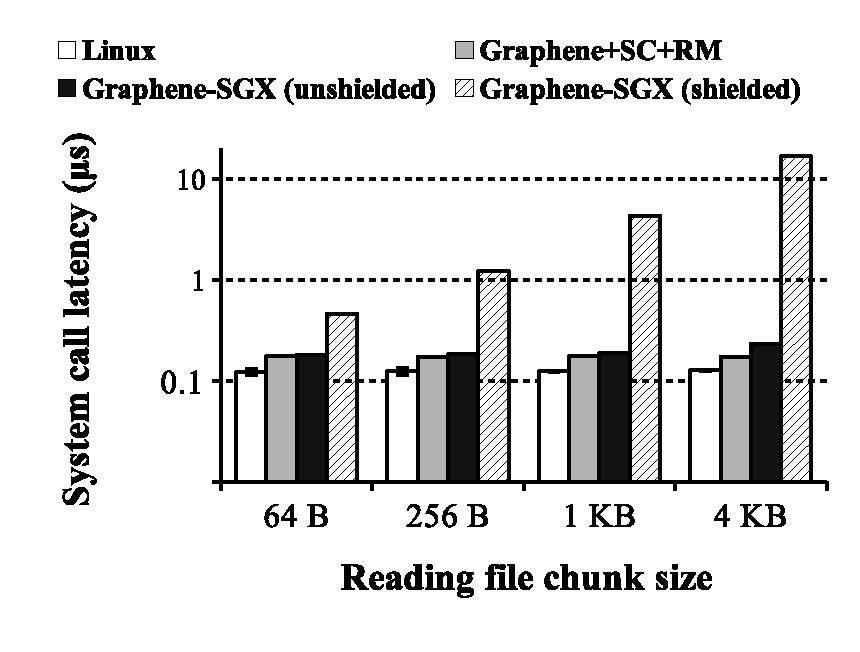
\includegraphics[height=10em]{pal/read-latency}
\quad
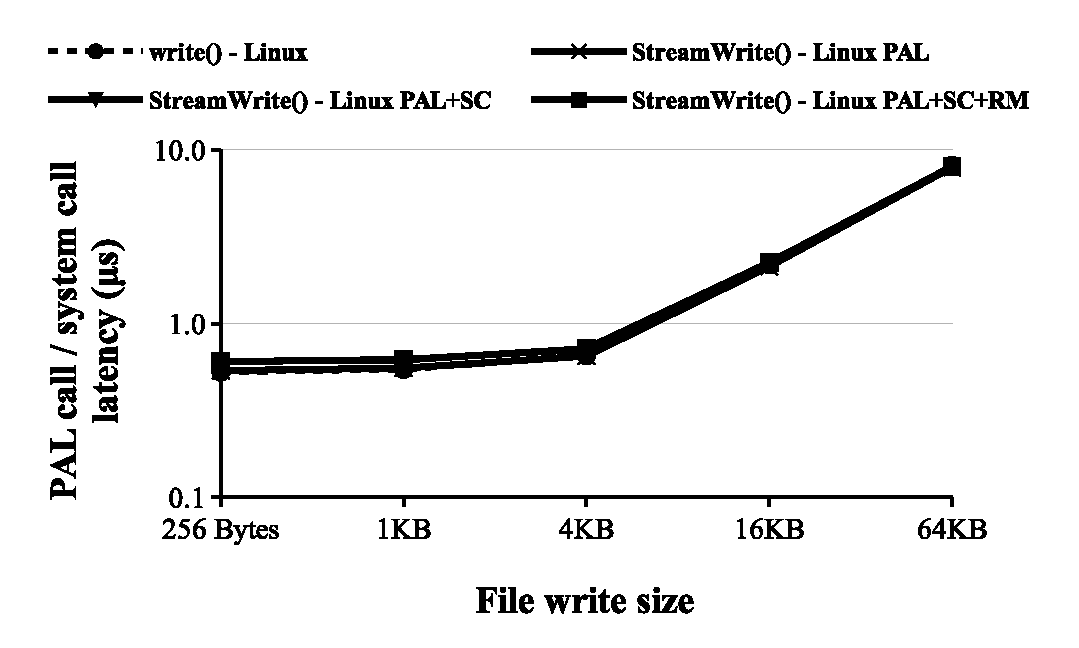
\includegraphics[height=10em]{pal/write-latency}
}
\parbox{0.49\textwidth}{\centering\bf (a) Sequential read}
\parbox{0.49\textwidth}{\centering\bf (b) Sequential write}
\caption{Latency of sequential \palcall{StreamRead} and \palcall{StreamWrite} on the Linux PAL,
versus \syscall{read} and \syscall{write} on Linux.
Lower is better.
Figure (a) and (b) respectively compares \palcall{StreamRead} and \palcall{StreamWrite} on the Linux PAL,
with and without a \seccomp{} filter ({\bf +SC})
and reference monitor ({\bf +RM}), against \syscall{read} and \syscall{write} on Linux.}
\label{fig:eval:pal:read-write-latency}
\end{figure*}





On the SGX PAL, as shown in
Figure~\ref{fig:eval:pal:sgx-read-write-latency} (a) and (b), the latency of sequential reads and writes
is dominated by the following overheads:
(1) copying the contents between the enclave and the untrusted PAL; (2) cryptographic operations for 
integrity checks. Without integrity checks,
the cost of exiting the enclave
and copying the contents across the enclave boundary is
8--12 \usec{} for reads and 8--50 \usec{} for writes.
For \palcall{StreamRead},
the SGX PAL checks the integrity of file contents
by comparing the secure hashes of 16KB blocks
against a Merkle tree constructed at \palcall{StreamOpen}.
\palcall{StreamRead}
always maps the file contents outside the enclave
in the multiple of 16KB,
and hashes the file contents after copy.
As a result, when the read size is smaller than 16KB,
the latency of \palcall{StreamRead} is constant.
Otherwise,
the latency of \palcall{StreamRead}
is proportional to the number of 16KB blocks read and checked by the SGX PAL.
\palcall{StreamWrite} is currently not protected by integrity checks on the SGX PAL.
%The integrity protection for contents written to a host file is not yet implemented in \graphenesgx{}.



\begin{figure*}[t!]
\centering
\footnotesize
\resizebox{\textwidth}{!}{%
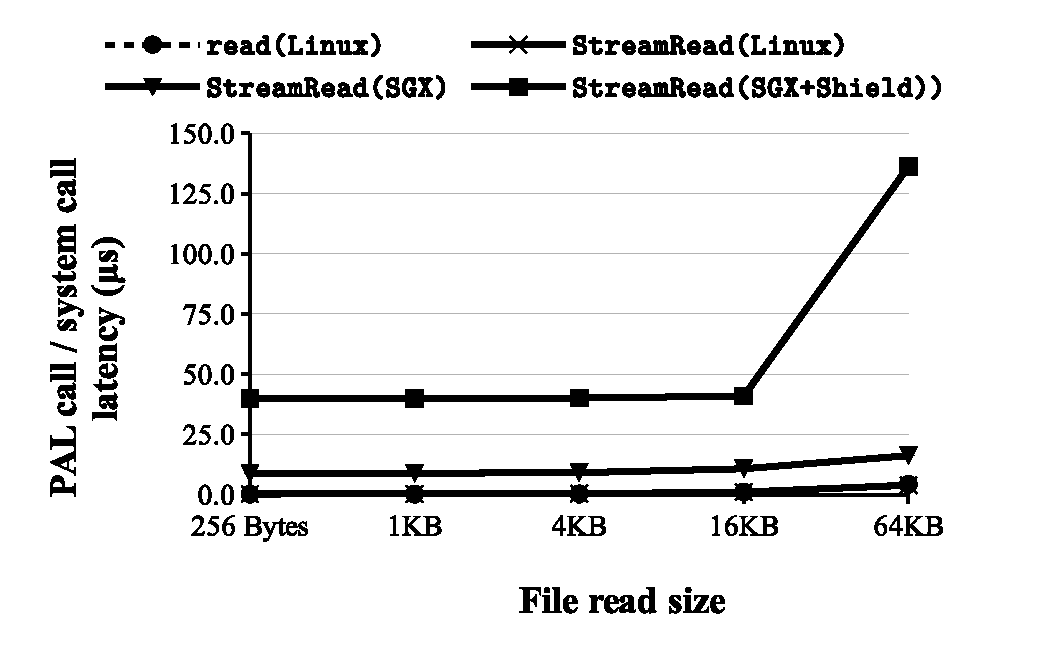
\includegraphics[height=10em]{pal/sgx-read-latency}
\quad
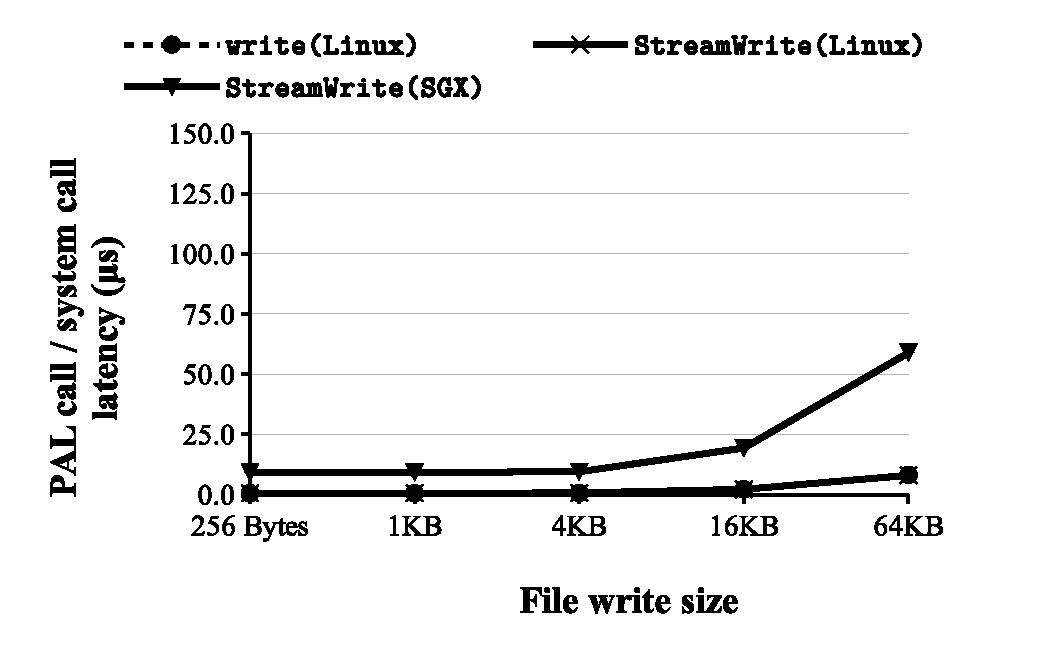
\includegraphics[height=10em]{pal/sgx-write-latency}
}
\parbox{0.49\textwidth}{\centering\bf (a) Sequential read}
\parbox{0.49\textwidth}{\centering\bf (b) Sequential write}
\caption{Latency of sequential \palcall{StreamRead} and \palcall{StreamWrite} on the SGX PAL,
versus the Linux PAL and Linux.
Lower is better.
Figure (a) and (b) respectively compares \palcall{StreamRead} and \palcall{StreamWrite} on the SGX PAL,
with and without integrity checks ({\bf +CHK})
and reference monitor ({\bf +RM}), against the Linux PAL and \syscall{read} and \syscall{write} on Linux. The current design does not support integrity checks for \palcall{StreamWrite}.}
\label{fig:eval:pal:sgx-read-write-latency}
\end{figure*}




%\paragraph{Network connections.}





\paragraph{TCP and UDP sockets.}
The evaluation shows both the latency and bandwidth of sending and receiving messages over a TCP or UDP sockets.
Figure~\ref{fig:eval:pal:network-latency-bandwidth} (a) shows the turnaround time of sending single-byte messages back and forth over a TCP or UDP stream (connected through the local loopback device), and
Figure~\ref{fig:eval:pal:network-latency-bandwidth} (b)
shows the bandwidth of a TCP or UDP stream
to transfer
64KB messages between \picoprocs{}.
On the Linux PAL,
the overheads of ping-ponging over TCP or UDP primarily contribute to the translation cost between
the \hostapis{} to Linux \linuxapis{} (specifically, \syscall{sendmsg} and \syscall{recvmsg}),
since the the \hostapis{} use strings as the network URIs and the Linux \linuxapis{} take a network address structure (\code{struct sockaddr}) that contains numeric representations in integers.
The translation costs for a TCP stream and a UDP stream are \roughly{}18\% and \roughly{}30\%, respectively.
The overhead is relatively marginal in the TCP bandwidth test,
at \roughly{}4\%.
Both the \seccomp{} filter and reference monitor adds
a marginal, less than 1\% overhead
to either the latency or bandwidth of TCP or UDP sockets.


On the SGX PAL, as shown in
Figure~\ref{fig:eval:pal:network-latency-bandwidth} (a) and (b),
both the latency and bandwidth of a network stream suffer significant overheads, mostly due to enclave exits and copying network payloads inside or outside of the enclave. Note that \graphenesgx{} assumes most applications are easily configured with TLS/SSL to protect the confidentiality and integrity of network payloads; therefore, the SGX PAL currently does not implement data protection for network sockets. The SGX PAL only checks the range of buffers
returned from the untrusted OS
to defend against pointer-based Iago attacks.
Without cryptographically protecting the messages, the overheads on TCP and UDP latency are \roughly{}167\% and \roughly{}131\%, respectively, and the overhead on TCP bandwidth is \roughly{}79\%. 

\begin{figure*}[t!]
\centering
\footnotesize
\resizebox{\textwidth}{!}{%
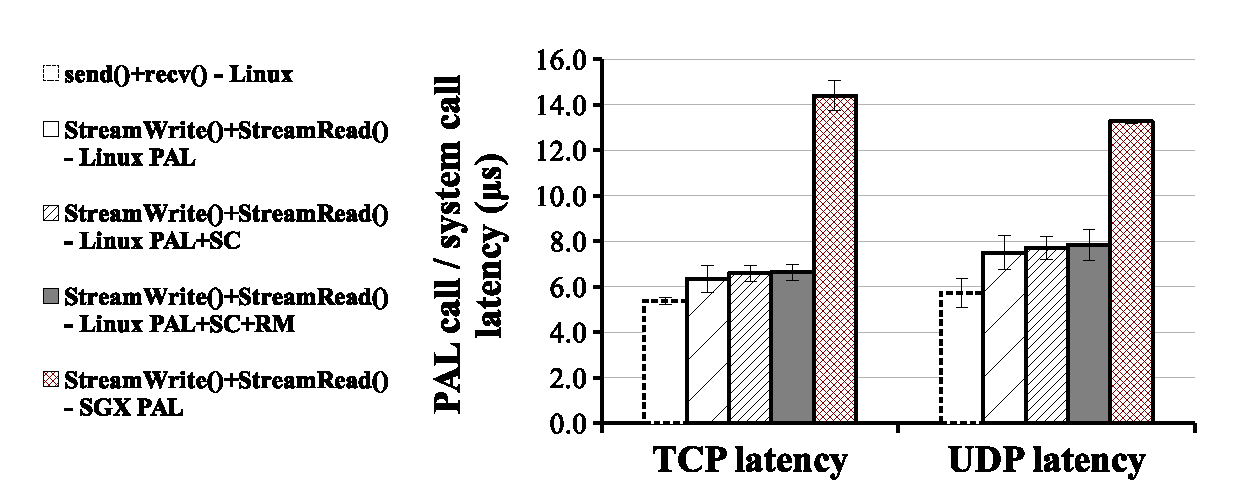
\includegraphics[height=10em]{pal/tcp-udp-latency}
\quad
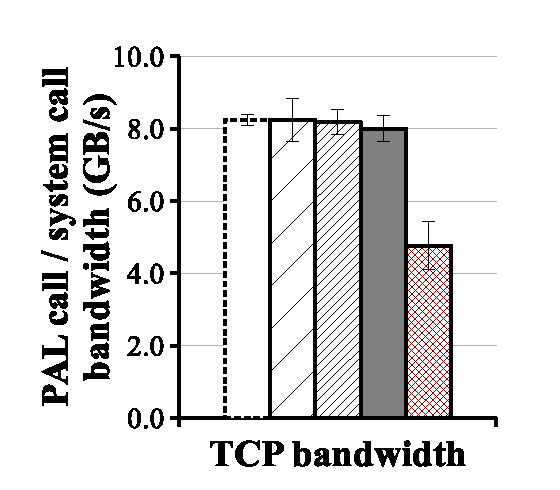
\includegraphics[height=10em]{pal/tcp-bandwidth}
}
\parbox{0.24\textwidth}{\quad}
\parbox{0.49\textwidth}{\centering\bf (a) Latency ({\usec})}
\parbox{0.24\textwidth}{\centering\bf (b) Bandwidth (MB/\asec{})}
\caption{(a) Latency of sending a short message over TCP and UDP sockets (lower is better), and (b) bandwidth of sending large data over TCP (higher is better).
The comparison is between (1) \syscall{recv} and \syscall{send} on Linux; (2) \palcall{StreamRead} and \palcall{StreamWrite} on a Linux PAL, with and without a \seccomp{} filter ({\bf +SC}) and reference monitor ({\bf +RM}); (3) the same \hostapis{} on the SGX PAL, without data protection.}
\label{fig:eval:pal:network-latency-bandwidth}
\end{figure*}




\paragraph{RPC latency and bandwidth.}
The evaluation shows the latency and bandwidth of using a RPC stream to send messages across \picoprocs{}.
Figure~\ref{fig:eval:pal:pipe-latency-bandwidth} (a) shows
the turnaround time of sending single-byte messages over a local RPC stream, and Figure~\ref{fig:eval:pal:pipe-latency-bandwidth} (a) shows the bandwidth of the RPC stream to send
64KB messages.
The evaluation also includes the latency and bandwidth of an unnamed pipe and a named UNIX domain socket
for comparison.
For the Linux PAL, the latency and bandwidth of a RPC stream is
close to a UNIX domain socket, due to the choice of underlying implementation.
Note that the evaluation results are specific to latest Linux kernels, especially kernels after 4.2,
which introduce a zero-copy UNIX network socket design. 
Both the \seccomp{} filter and reference monitor have marginal overhead on latency and bandwidth.


For the SGX PAL,
the fundamental cost of enclave exits and copying message contents,
without protecting the message contents,
is \roughly{}154\% to the latency,
or \roughly{}127\% to the bandwidth.
However, unlike network streams, \graphenesgx{} cannot assume RPC streams to be protected by inlined SSL/TLS connections
inside applications.
Since it is likely that an application may send sensitive information
over a pipe or a UNIX socket,
the underlying RPC streams must always be protected by the SGX PAL.
For each RPC streams, the SGX PAL establishes a TLS connection using a AES-GCM algorithm, which both authenticates and encrypts the message contents.
The AES-GCM algorithm in \graphenesgx{} is accelerated by the Intel AES-NI instructions, which are guaranteed to exist on a SGX-enabled CPU.
With the hardware-accelerated AES-GCM,
the overhead on the RPC latency is still up to \roughly{}335\% compared to the UNIX domain socket;
furthermore, RPC bandwidth
is reduced by \roughly{}20$\times$, at \roughly{}0.3 GB/s.
Potentially switching to a more efficient cryptographic algorithm or library may improve the overheads on RPC streams,
and the experiment is left for future work.



\begin{figure*}[t!]
\centering
\footnotesize
\resizebox{\textwidth}{!}{%
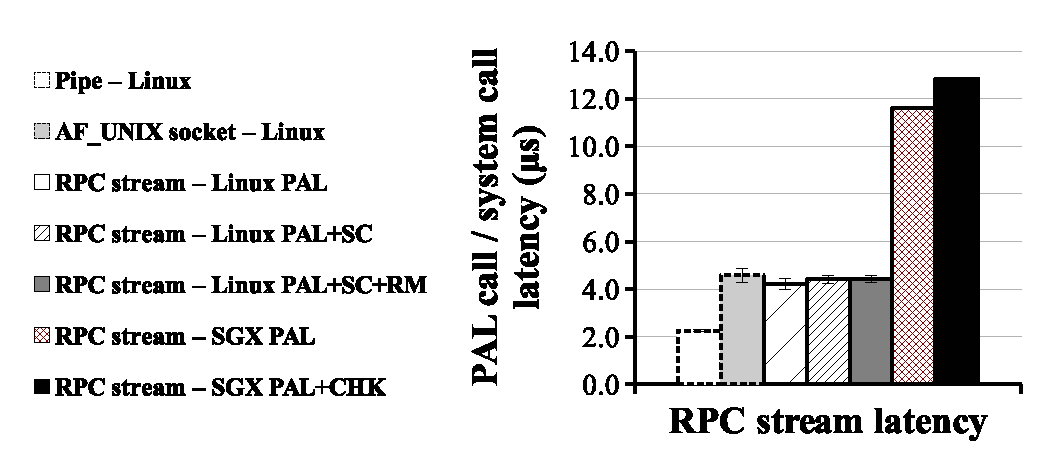
\includegraphics[height=10em]{pal/pipe-latency}
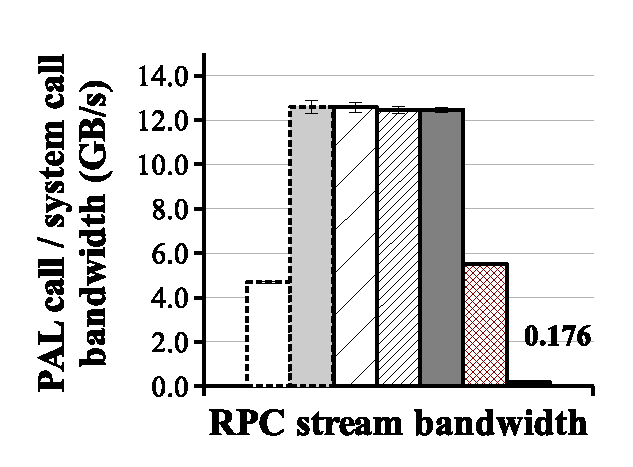
\includegraphics[height=10em]{pal/pipe-bandwidth}
}
\parbox{0.30\textwidth}{\quad}
\parbox{0.34\textwidth}{\centering\bf (a) Latency ({\usec})}
\parbox{0.34\textwidth}{\centering\bf (b) Bandwidth (MB/\asec{})}
\caption{(a) Latency of sending a short message over RPC (lower is better), and (b) bandwidth of sending large data (higher is better).
The comparison is between (1) \syscall{read} and \syscall{write} over a pipe or an AF\_UNIX socket on Linux; (2) \palcall{StreamRead} and \palcall{StreamWrite} on the Linux PAL, with and without a \seccomp{} filter ({\bf +SC}) and reference monitor ({\bf +RM}); (3) the same \hostapis{} on the SGX PAL, with and without data protection ({\bf +CHK}).}
\label{fig:eval:pal:pipe-latency-bandwidth}
\end{figure*}


\paragraph{Summary.}
The efficiency of \hostapis{} for accessing files or I/O streams
inevitably suffers some overheads,
due to the nature of these abstractions to be sharable
among applications.
Each of these \hostapis{} externalizes certain guest OS states
%such as buffered file contents or network payloads,
to the host OS,
using the existing host system interfaces.
Most of the experiment results
show that the translation cost between the \hostapis{} and the host system interfaces can be reduced
by mitigating the needs of reconstructing the \hostapi{} arguments
and copying stream buffers.
Only a few exceptions, such as the translation of URIs to network addresses,
or copying the arguments or buffers in or out of an enclave,
cause more significant overheads to the overhead of these \linuxapis{}.




Security checks, either in the host kernel or inside an enclave,
often contribute to
non-trivial overheads on the \hostapis{} for accessing I/O streams.
The cost of security checks
varies between different threat models.
For the Linux PAL, the cost includes the overhead of enabling a \seccomp{} filter, and the cost of checking file paths and network addresses
inside of an reference monitor.
With the JIT (Just-in-time) optimization,
the overheads of \seccomp{} filter is generally less than 10\%.
The overheads of security monitors can range from 0--21\%, but only impact \hostapis{} which accept an URI as argument (e.g., \palcall{StreamOpen} and \palcall{StreamAttrQuery}).

 
The SGX PAL further adopts several cryptographic techniques
for protecting the confidentiality and integrity of I/O streams, which impose significant overheads.
Verifying the file contents, either at first open of the file or consequential file reads,
causes 500--24,000$\times$ overheads on \palcall{StreamOpen}
or 25--150$\times$ overheads on \palcall{StreamRead}.
Authenticating and encrypting a RPC stream, using a TLS connection with hardware-accelerated AES-GCM algorithm,
causes \roughly{}335\% overhead beyond the latency of underlying UNIX domain sockets,
or \roughly{}20 $\times$ overhead on bandwidth when sending large messages.






\subsection{Page management}


Figure~\ref{fig:eval:pal:mmap-latency} (a)
shows the combined latency of \palcall{VirtMemAlloc} and  \palcall{VirtMemFree}, on both Linux and SGX PALs,
and the latency of \syscall{mmap} and \syscall{munmap} in a native Linux process.
The latency of both \syscall{mmap}+\syscall{munmap} and \syscall{VirtMemAlloc}+\syscall{VirtMemFree} on Linux is partially correlated with the size of memory mapped inside a process or \picoproc{}.
Due to the similarity between the \hostapis{} and the \linuxapis{},
the translation cost is almost marginal
to the latency of allocating and deallocating the memory mappings.
Enabling the \seccomp{} filter adds an additional
15--25\% overhead to the latency of \syscall{VirtMemAlloc}+\syscall{VirtMemFree}, which is common for all \linuxapis{} used by the Linux PAL.
However, if the latency includes zeroing the allocated memory mappings,
which triggers the population of physical pages
inside the host kernel,
the overhead is much more significant and proportional to the mapping size.
As a result, allocating, accessing, and deallocating a 64MB memory mapping will take up to \roughly{}3.5\msec{}.


For the SGX PAL, the latency of allocating and deallocating memory mapping
is much lower then the Linux PAL, because the SGX PAL does not dynamically allocate the enclave memory region.
Due the limitation of current SGX hardware,
the SGX PAL must implement memory mappings internally,
with all the enclave page populated and signed by the CPU before the enclave starts execution.
Based on this design, the latency of \syscall{VirtMemAlloc}+\syscall{VirtMemFree} on the SGX PAL
is 8--11\% of the latency on the Linux PAL,
since these two \hostapis{} only update the memory mapping records inside the enclave.
However, if the enclave memory is accessed immediately after allocation, as shown in Figure~\ref{fig:eval:pal:mmap-latency} (b),
the overhead can be up to 3--9.5$\times$, and is proportional to the size of memory mappings.

\begin{figure*}[t!]
\centering
\footnotesize
\resizebox{\textwidth}{!}{%
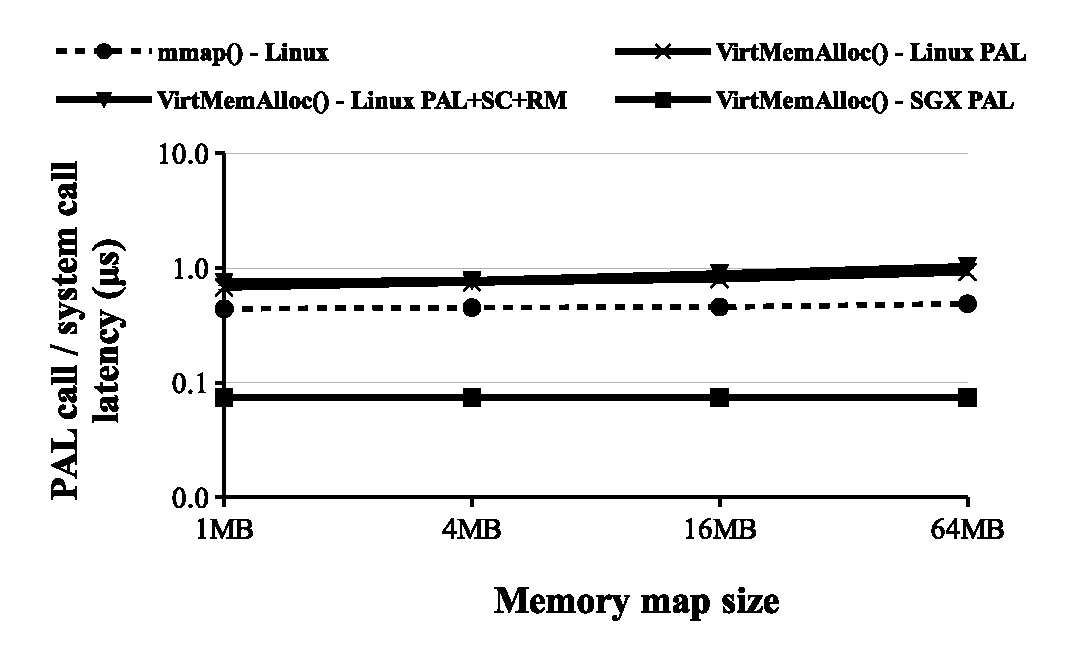
\includegraphics[height=10em]{pal/mmap-latency}
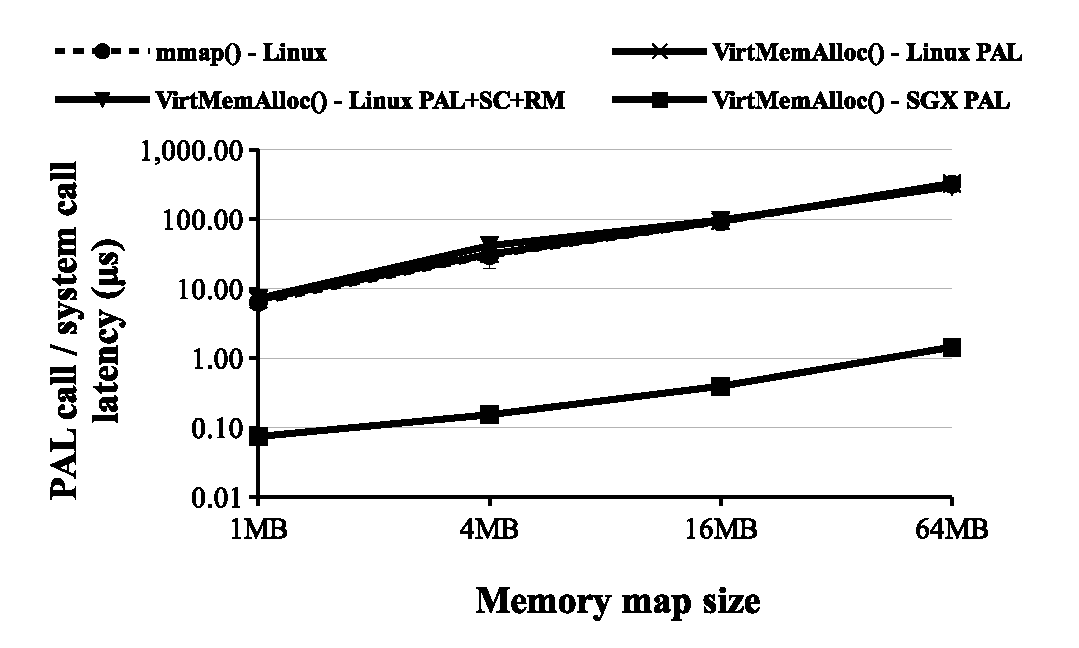
\includegraphics[height=10em]{pal/mmap-access-latency}
}
\parbox{0.49\textwidth}{\centering\bf (a) allocation + deallocation}
\parbox{0.49\textwidth}{\centering\bf (b) allocation + memory access + deallocation}
\caption{Latency of (a) allocating and deallocating a range of virtual pages, and (b) the same operations with writing to each page after allocation. Lower is better.
The comparison is between (1) \syscall{mmap} and \syscall{munmap} on Linux; (2) \palcall{VirtMemAlloc} and \palcall{VirtMemFree} on the Linux PAL, with and without a \seccomp{} filter ({\bf +SC}) and reference monitor ({\bf +RM}); (3) the same \hostapis{} on the SGX PAL, with and without zeroing the pages before use ({\bf +Zero}).}
\label{fig:eval:pal:mmap-latency}
\end{figure*}


The evaluation results on \syscall{VirtMemAlloc} and \syscall{VirtMemFree}
show that the Linux PAL share the same latency
with a native Linux process
for creating virtual memory mappings, paging and memory access.
On the other hand, despite that the SGX PAL manages all the enclave pages
inside the enclave,
the SGX PAL suffers a larger overhead for paging and bringing memory into the last-level cache.



\subsection{Scheduling}




\begin{figure*}[t!]
\centering
\footnotesize
\resizebox{\textwidth}{!}{%
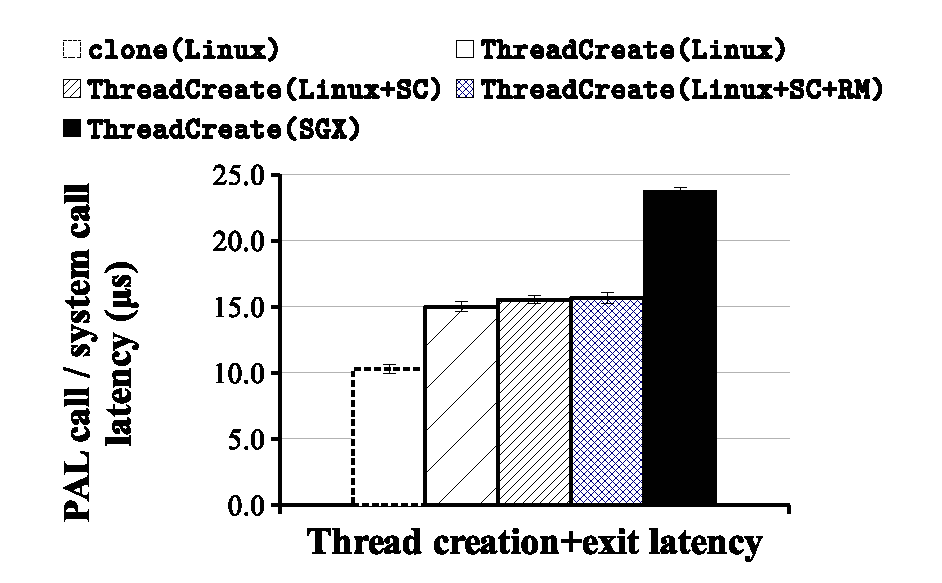
\includegraphics[height=10em]{pal/thread-latency}
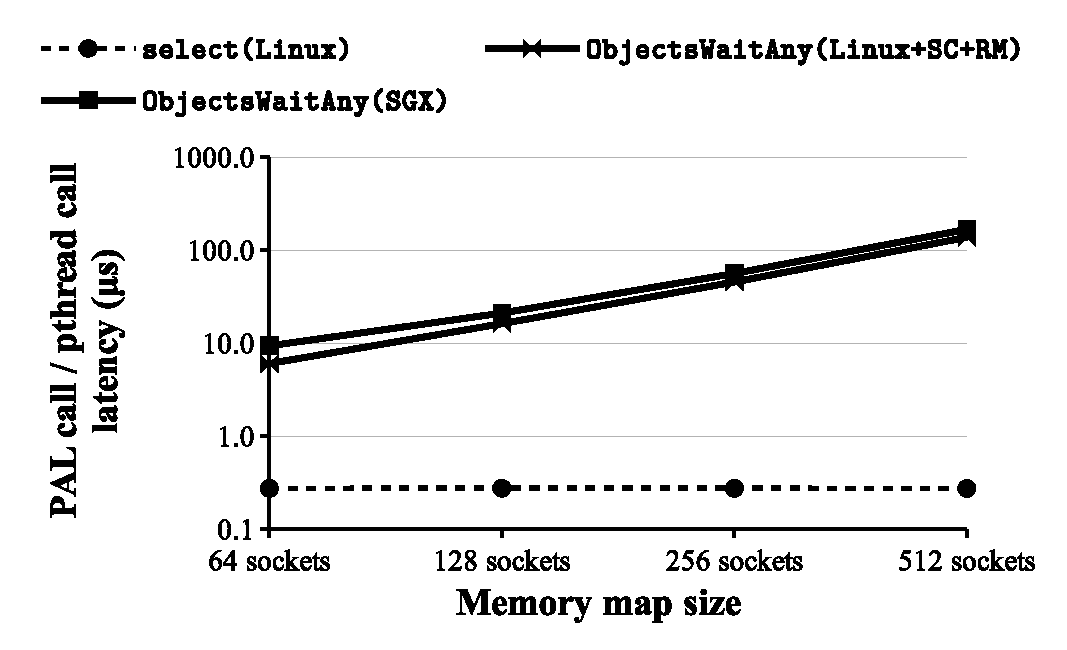
\includegraphics[height=10em]{pal/tcp-select-latency}
}
\parbox{0.49\textwidth}{\centering\bf (a) thread creation}
\parbox{0.49\textwidth}{\centering\bf (b) polling N TCP sockets}
\caption{(a) Thread creation latency and (b) latency of polling a number of TCP sockets.
Lower is better.
The comparison is between (1) \syscall{clone} and \syscall{select} on Linux; (2) \palcall{ThreadCreate} and \palcall{ObjectsWaitAny} on the Linux PAL, with and without a \seccomp{} filter ({\bf +SC}) and reference monitor ({\bf +RM}); (3) the same \hostapis{} on the SGX PAL.}
\label{fig:eval:pal:thread-select-latency}
\end{figure*}


\paragraph{Thread creation.}



\paragraph{Polling stream handles.}




\begin{figure*}[t!]
\centering
\footnotesize
\resizebox{\textwidth}{!}{%
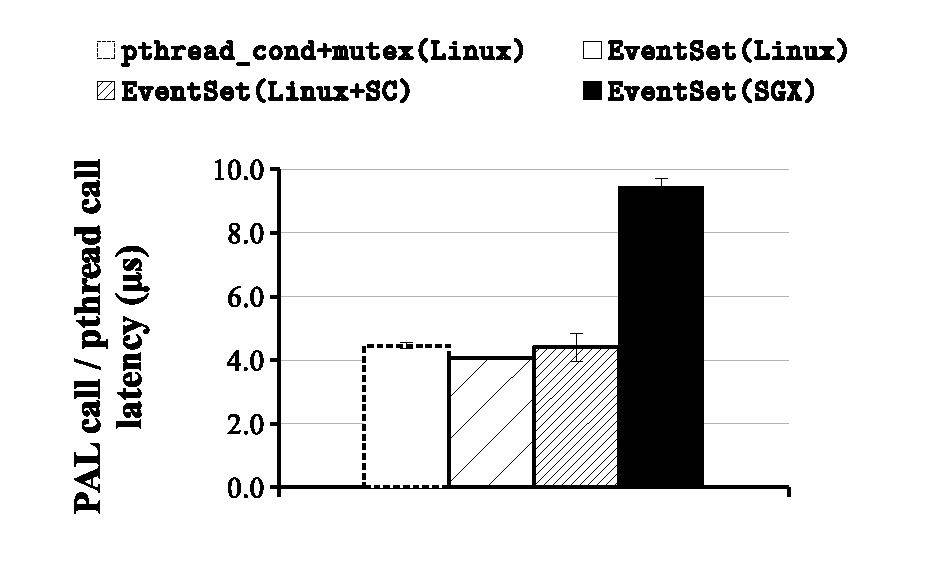
\includegraphics[height=10em]{pal/event-latency}
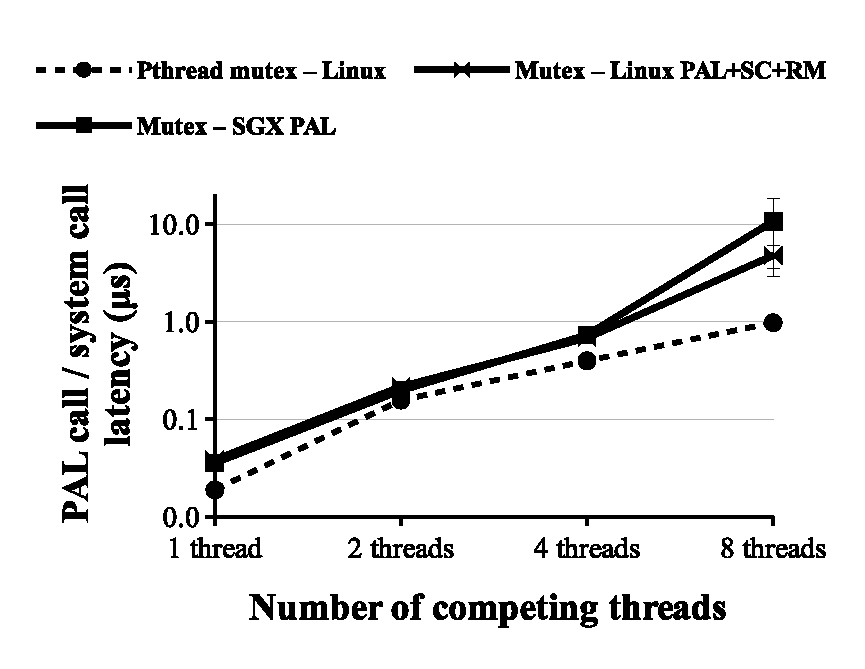
\includegraphics[height=10em]{pal/mutex-latency}
}
\parbox{0.49\textwidth}{\centering\bf (a) signal an event}
\parbox{0.49\textwidth}{\centering\bf (b) competing a mutex among N threads}
\caption{Latency of (a) signaling an event and (b) competing a mutex among N threads (N: 1 to 8).
Lower is better.
The comparison is between (1) pthread condition variables and mutexes on Linux; (2) Notification events and mutexes on the Linux PAL, with and without a \seccomp{} filter ({\bf +SC}) and reference monitor ({\bf +RM}); (3) the same abstractions on the SGX PAL.}
\label{fig:eval:pal:sched-latency}
\end{figure*}



\paragraph{Events and mutexes.}


\subsection{Multi-process abstractions}


\begin{figure*}[t!]
\centering
\footnotesize
\resizebox{\textwidth}{!}{%
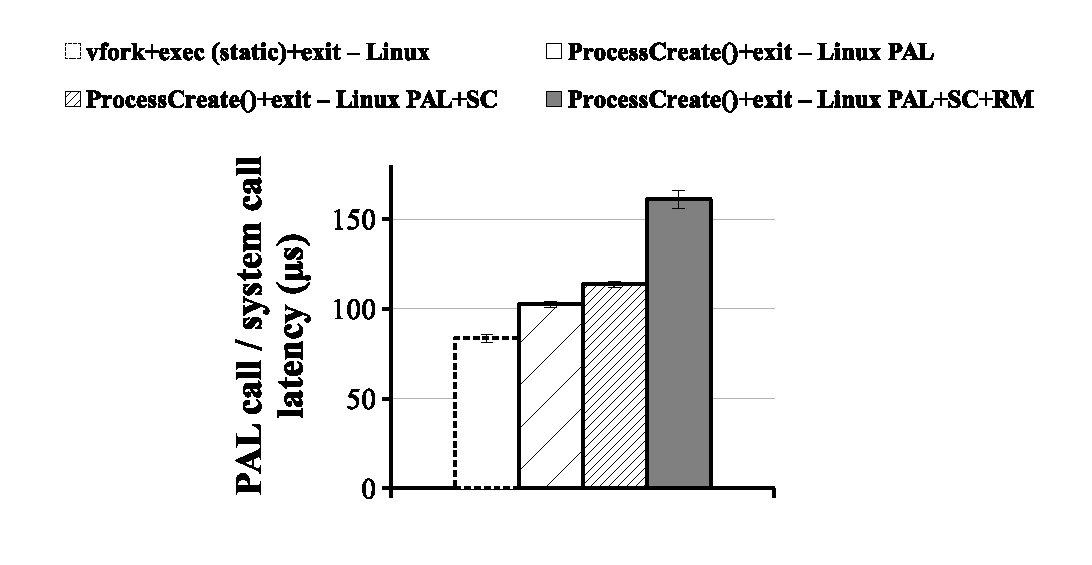
\includegraphics[height=10em]{pal/proc-latency}
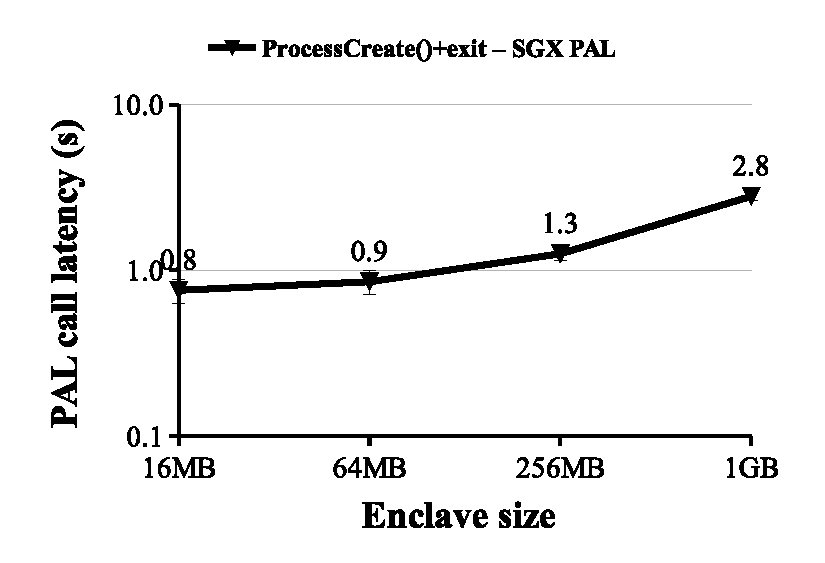
\includegraphics[height=10em]{pal/sgx-proc-latency}
}
\parbox{0.59\textwidth}{\centering\bf (a) process creation+exit}
\parbox{0.39\textwidth}{\centering\bf (b) SGX enclave creation+termination}
\caption{Latency of creating (a) a clean process on the Linux PAL, and (b) an enclave on the SGX PAL, in respect of different enclave sizes.
The comparison is between (1) a combination of \syscall{vfork} and \syscall{exec}'ing a minimal static program on Linux; (2) \palcall{ProcessCreate} on the Linux PAL, with and without a \seccomp{} filter ({\bf +SC}) and reference monitor ({\bf +RM}); (3) the same \hostapi{} on the SGX PAL.}
\label{fig:eval:pal:proc-latency}
\end{figure*}

\paragraph{Process creation.}




\begin{figure*}[t!]
\centering
\footnotesize
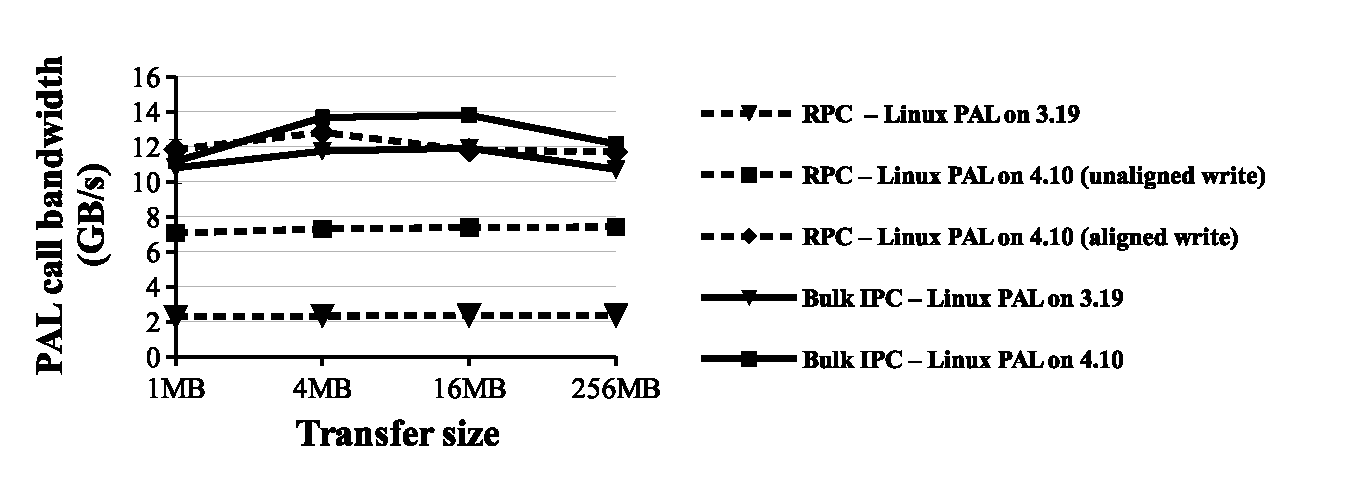
\includegraphics[width=.85\textwidth]{pal/gipc-bandwidth}
\caption{Bandwidth of sending large messages over (a) RPC streams and (b) Bulk IPC channels. The messages are sent in different sizes (1MB to 256MB), and either aligned or unaligned with the page boundary.
Higher is better. Both abstractions are benchmarked on Linux kernel 3.19 and 4.10 as the hosts. The impact of the \seccomp{} filter or reference monitor is marginal (less than 1\%).}
\label{fig:eval:pal:gipc-bandwidth}
\end{figure*}


\paragraph{Bulk IPC vs RPC streams.}




\subsection{Exception handling}


\begin{figure*}[t!]
\centering
\footnotesize
\resizebox{\textwidth}{!}{%
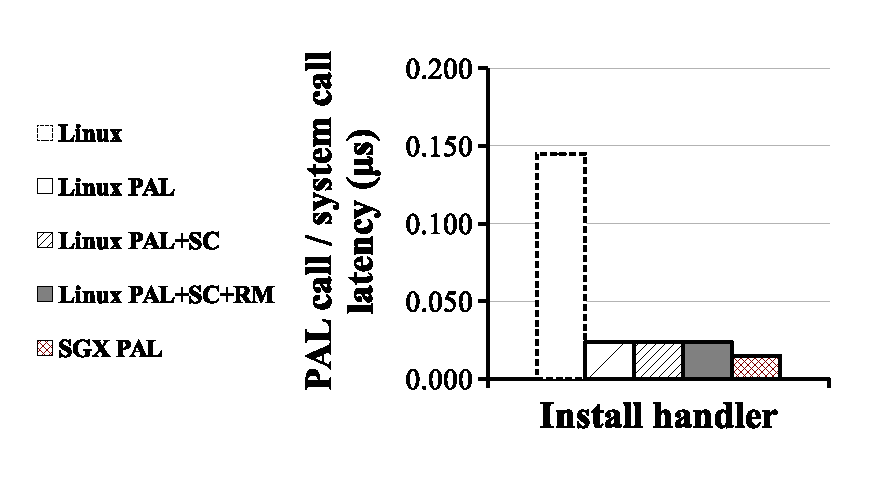
\includegraphics[height=10em]{pal/sig-install-latency}
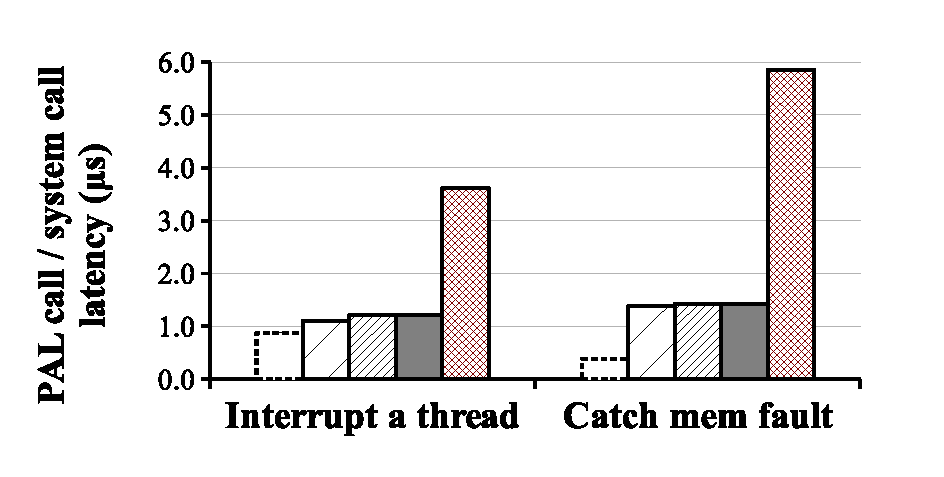
\includegraphics[height=10em]{pal/sig-catch-latency}
}
\caption{Latency of (a) installing an exception handler; (b)
interrupting a running thread with signals (on Linux) or \palcall{ThreadInterrupt} on the PALs; (c) catching a memory protection fault. Lower is better. The comparison is between (1) signals on Linux; (2) the Linux PAL, with and without a \seccomp{} filter ({\bf +SC}) and reference monitor ({\bf +RM}); (3) the SGX PAL.}
\label{fig:eval:pal:sig-latency}
\end{figure*}